%------------------------------------------
%	$Id$
%
%	The GMT Documentation Project
%	Copyright (c) 2000-2012.
%	P. Wessel, W. H. F. Smith, R. Scharroo, and J. Luis
%------------------------------------------
%

\chapter{Including \gmt\ graphics into your documents}
\thispagestyle{headings}
\label{app:C}
\index{GMT@\GMT!graphics in documents}
\index{Documents!include GMT@\GMT\ graphics}

Now that you made some nice graphics with \GMT, it is time to add them to a document, an article, a report, your dissertation, a poster, a web page, or a presentation. Of course, you could try the old-fashioned scissors and glue stick. More likely, you want to incorporate your graphics electronically into the document. Depending on the application, the \GMT\ \PS\ file will need to be converted to Encapsulated \PS\ (EPS), Portable Document Format (PDF), or some raster format (e.g., JPEG, PNG, or TIFF) in order to incorporate them into the document.
\begin{itemize}
\item When creating a document intended for printing (article, dissertation, or poster) it is best to preserve the scalable vector characteristics of the \PS\ file. Many applications can directly incorporate \PS\ in the form of EPS files. Modern programs will often allow the inclusion of PDF files. Either way, the sharpness of lines and fonts will be preserved and can be scaled up or down as required.
\item When the aim is to display the graphics on a computer screen or present it using a projector, it is wise to convert the \PS\ into a raster format. Although applications like \progname{PowerPoint} can do this for you, you can best take the conversion into your own hands for the best results.
\end{itemize}
A large number of questions to the GMT-Help mailing list are related to these rendering issues, showing that something as seemingly straightforward as incorporating a \PS\ file into a document is a far from trivial exercise.
This Chapter will show how to include \GMT\ graphics into documents and how to achieve the best quality results.

\section{Making \gmt\ Encapsulated \PS\ Files}
\label{sec:eps}
\index{PostScript@\PS!encapsulated (EPS)}
\index{PostScript@\PS!BoundingBox}
\index{EPS file}

\GMT\ can produce both freeform \PS\ files and the more restricted Encapsulated \PS\ files (EPS).  The former is intended to be sent to a printer or \PS\ previewer,
while the latter is intended to be included in another document (but should also be able to print and preview).  You control what kind of \PS\ that \GMT\ produces by
manipulating the \textbf{PS\_MEDIA} parameter (see the \GMTprog{gmt.conf} man page for how this is accomplished).  Note that a freeform \PS\ file may contain special operators (such as \texttt{Setpagedevice}) that is specific to printers (e.g., selection of paper tray). Some previewers (among them, Sun's \progname{pageview}) do not understand these valid instructions and may fail to image the file. Also, embedding freeform \PS\ with such instructions in it into a larger document can create printing to fail. While you could choose another viewer (we recommend \progname {ghostview}) to view single plots prepared by \GMT, it is generally wiser anyhow to select EPS output when you are creating a plot intended for inclusion into a larger document. Some programs (and some publishers as well) do not allow the use of instructions like \texttt{Setpagedevice} as part of embedded graphics.

An EPS file that is to be placed into another document needs to have correct bounding box parameters.  These are found in the \PS\ Document Comment \%\%BoundingBox.  Applications that generate EPS files should set these parameters correctly.  Because \GMT\
makes the \PS\ files on the fly, often with several overlays, it is not possible to do so accurately.  However, \GMT\ does make an effort to ensure that the BoundingBox is large enough to contain the entire composite plot\footnote{In contrast, regular \GMT\ \PS\ files simply have a \%\%BoundingBox that equal the size of the chosen paper.}. Therefore, if you need a ``tight'' BoundingBox you need to post-process your \PS\ file.  There are several ways in which this can be accomplished.

\begin{itemize}
\item Programs such as Adobe \progname{Illustrator}, Aldus \progname{Freehand}, and Corel \progname{Draw} will allow you to edit the BoundingBox graphically.

\item A command-line alternative is to use freely-available program \progname{epstool} from the makers of Aladdin \progname{ghostscript}.  Running
\small
\begin{verbatim}
epstool -c -b myplot.ps
\end{verbatim}
\normalsize
should give a tight BoundingBox; \progname{epstool} assumes the plot is page size and not a huge poster.

\item Another option is to use \progname{ps2epsi} which also comes with the \progname{ghostscript} package.  Running
\small
\begin{verbatim}
ps2epsi myplot.ps myplot.eps
\end{verbatim}
\normalsize
should also do the trick. The downside is that this program adds an ``image'' of the plot in the preamble of the EPS file, thus increasing the file size significantly. This image is a rough rendering of your \PS\ graphics that some programs will show on screen while you are editing your document. This image is basically a placeholder for the \PS\ graphics that will actually be printed.

\item The preferred option is to use the \GMT\ utility \GMTprog{ps2raster}. Its \Opt{A} option will figure out the tightest BoundingBox, again using \progname{ghostscript} in the background. For example, running
\small
\begin{verbatim}
ps2raster -A -Te myplot.ps
\end{verbatim}
\normalsize
will convert the \PS\ file \filename{myplot.ps} into an encapsulated \PS\ file \filename{myplot.eps} which is exactly cropped to the tightest possible BoundingBox.
\end{itemize}

If you do not want to modify your illustration but just include it in a text document: many word processors (such as Microsoft \progname{Word}, Corel \progname{WordPerfect}, and Apple \progname{Pages}) will let you include a \PS\ file that you may place but not edit. Newer versions of those programs also allow you to include PDF versions of your graphics. Except for \progname{Pages}, 
you will not be able to view the figure on-screen, but it will print correctly.

\section{Converting \gmt\ \PS\ to PDF or raster images}
\index{PostScript@\PS!convert to PDF}
\index{PDF file}
\index{PostScript@\PS!convert to raster image}
\index{PNG file}
\index{PostScript@\PS!rendering}

Since Adobe's PDF (Portable Document Format) seems to become the \emph{de facto} standard for vector graphics, you are often well off converting \GMT\ produced \PS\ files to PDF. Being both vector formats (i.e., they basically describe all objects, text and graphics as lines and curves), such conversion sounds awfully straightforward and not worth a full section in this document. But experience has shown differently, since most converters cut corners by using the same tool (Aladdin's \progname{ghostscript}) with basic default options that are not devised to produce the best quality PDF files.

For some applications it is practical or even essential that you convert your \PS\ file into a raster format, such as GIF (Graphics Interchange Format), TIFF (Tagged Image File Format), PNG (Portable Network Graphics), or JPEG (Joint Photographic Experts Group). A web page is better served with a raster image that will immediately show on a web browser, than with a \PS\ file that needs to be downloaded to view, despite the better printing quality of the \PS\ image. A less obvious reason to convert your image to a raster format is to by-pass \progname{PowerPoint}'s rendering engine in case you want to embed the image into a presentation.

The are a number of programs that will convert \PS\ files to PDF or raster formats, like Aladdin's \progname{pstopdf}, pbmplus' \progname{pstoimg}, or ImageMagick's \progname{convert}, most of which run \progname{ghostscript} behind the scenes. The same is true for viewers like \progname{ghostview} and Apple's \progname{Preview}. So a lot of the times when people report that their \PS\ plot does not look right but prints fine, it is the way \progname{ghostscript} is used with its most basic settings that is to blame.

\subsection{When converting or viewing \PS\ goes awry}
\index{Anti-aliasing}
\index{Image compression!lossy and non-lossy}
\index{Font!including in PDF}
Here are some notorious pitfalls with \progname{ghostscript} (and other rendering programs for that matter).
\begin{description}
\item[Rendering.] When you are converting to a raster format, make sure you use a high enough resolution so that the pixels do not show when it is enlarged onto a screen or using a projector. The right choice of resolution depends on the application, but do not feel limited to the default 72 dpi (dots-per-inch) that is offered by most converters.

\item[Image compression.] There are \emph{lossy} and \emph{non-lossy} compressions. A compression algorithm is called ``lossy'' when information is lost in the conversion: there is no way back to get the full original. The effect can be seen when there are sharp color transitions in your image: the edges will get blurry in order to allow a more efficient compression. JPEG uses a lossy compression, PNG is non-lossy, and TIFF generally does not use compression at all. We therefore recommend you convert to PNG if you need to rasterize your plot, and leave JPEG to photographs.

\item[Embedded image compression.] When your \GMT\ plot includes objects produced by \GMTprog{grdimage}, \GMTprog{psimage} or \GMTprog{pslegend}, they are seen as ``images''. The default options of \progname{ghostscript} will use a \emph{lossy} compression (similar to JPEG) on those images when converting them to PDF objects. This can be avoided, however, by inhibiting the compression altogether, or using the non-lossy \emph{flate} compression, similar to the one used in the old \progname{compress} program. This compression is fully reversible, so that your image does not suffer any loss.

\item[Auto-rotation.] The \progname{ghostscript} engine has the annoying habit to automatically rotate an image produced with portrait orientation (using the \Opt{P} option) so that the height is always larger than the width. So if you have an image that was printed in portrait mode but happens to have a width larger than height (for example a global map), it would suddenly get rotated. Again, this function needs to be switched off. Apple's \progname{Preview} uses the \progname{ghostscript} engine and suffers from the same annoying habit. Oddly enough, \progname{ghostscript} does not force landscape plots to be ``horizontal''.

\item[Anti-aliasing.] This is not something to worry about when converting to PDF, but certainly when producing raster images (discussed below). \emph{Anti-aliasing} in this context means that the rendering tries to avoid \emph{aliasing}, for example, sampling only the blacks in a black-and-white hachure. It does so by first oversampling the image and then using ``gray-shades'' when a target pixel is only partially white or black.

Clearly, this can lead to some unwanted results. First, all edges and lines get blurry and second, the assumption of a white background causes the gray shades to stand out when transferring the image to background with a different color (like the popular sleep-inducing blue in \progname{PowerPoint} presentations). A more surprising effect of anti-aliasing is that the seams between tiles that make up the land mask when using \GMTprog{pscoast} will become visible. The anti-aliasing somehow decides to blur the edges of all polygons, even when they are seamlessly connected to other polygons.

It is therefore wise to overrule the default anti-aliasing option and over-sample the image yourself by choosing a higher resolution.

\item[Including fonts.] When you are producing print-ready copy to publishers, they will often (and justifiably) ask that you include all fonts in your PDF document. Again, \progname{ghostscript} (and all converters relying on that engine) will not do so by default.
\end{description}

\subsection{Using \GMTprog{ps2raster}}

The remedy to all the problems mentioned in the previous section is readily available to you in the form of the \GMT\ utility \GMTprog{ps2raster}. It is designed to provide the best quality PDF and raster files using \progname{ghostscript} as a rendering engine. The program \GMTprog{ps2raster} avoids anti-aliasing and lossy compression techniques that are default to \progname{ghostscript} and includes the fonts into the resulting PDF file to ensure portability. By default the fonts are rendered at 720 dots-per-inch in a PDF file and images are sampled to 300 dpi, but that can be changed with the \Opt{E} option. Simply run
\small
\begin{verbatim}
ps2raster -A -P -Tf *.ps
\end{verbatim}
\normalsize
to convert all \PS\ files to PDF while cropping it to the smallest possible BoundingBox. Or use the \Opt{Tg} option to convert your files to PNG.

The \Opt{P} option of \GMTprog{ps2raster} may also come in handy. When you have \emph{not} supplied the \Opt{P} option in your first \GMT\ plot command, your plot will be in Landscape mode. That means that the plot will be rotated 90 degrees (anti-clockwise) to fit on a Portrait mode page when coming out of the printer. The \Opt{P} option of \GMTprog{ps2raster} will undo that rotation, so that you do not have to do so within your document. This will only affect Landscape plots; Portrait plots will not be rotated.

\section{Examples}
\subsection{\gmt\ graphics in \LaTeX}
\index{LaTeX@\LaTeX}
\index{includegraphics}

Nearly all illustrations in this \GMT\ documentation were \GMT-produced \PS\ files. They were converted to PDF files using \GMTprog{ps2raster} and then included into a \LaTeX\ document that was processed with \progname{pdflatex} to create the PDF document you are reading.

To add the graphics into the \LaTeX\ document we use the \verb|\includegraphics| command supplied by the \textsf{graphicx} package. In the preamble of your \LaTeX\ document you will need to include the line
\small
\begin{verbatim}
\usepackage{graphicx}
\end{verbatim}
\normalsize
The inclusion of the graphics will probably be inside a floating figure environment; something like this
\small
\begin{verbatim}
\begin{figure}
   \includegraphics{myplot}
   \caption{This is my first plot in \LaTeX.}
   \label{fig:myplot}
\end{figure}
\end{verbatim}
\normalsize
Note that the \verb|\includegraphics| command does not require you to add the suffix \verb|.pdf| to the file name. If you run \progname{pdflatex}, it will look automatically for \filename{myplot.pdf}. If you run \progname{latex}, it will use \filename{myplot.eps} instead.

You can scale your plot using the options \verb|width=|, \verb|height=|, or \verb|scale=|. In addition, if your original graphics was produced in Landscape mode (i.e., you did \emph{not} use \GMT's \Opt{P} option: not while plotting, nor in \GMTprog{ps2raster}), you will need to rotate the plot as well. For example,
\small
\begin{verbatim}
\includegraphics[angle=-90,width=0.8\textwidth]{myplot}
\end{verbatim}
\normalsize
will rotate the image 90\DS\ clockwise and scale it such that its width (after rotation) will be 80\% of the width of the text column.

\subsection{\gmt\ graphics in \protect\progname{PowerPoint}}
\begin{figure}[b]
   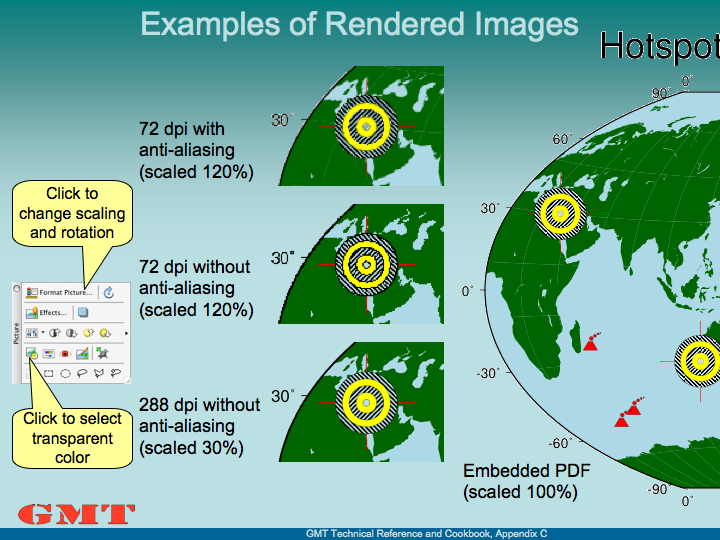
\includegraphics[width=\textwidth,bb=0 0 720 540]{rendering.png}
   \caption{Examples of rendered images in a \protect\progname{PowerPoint} presentation.}
   \label{fig:rendering}
\end{figure}
\begin{figure}[b]
   \centering
   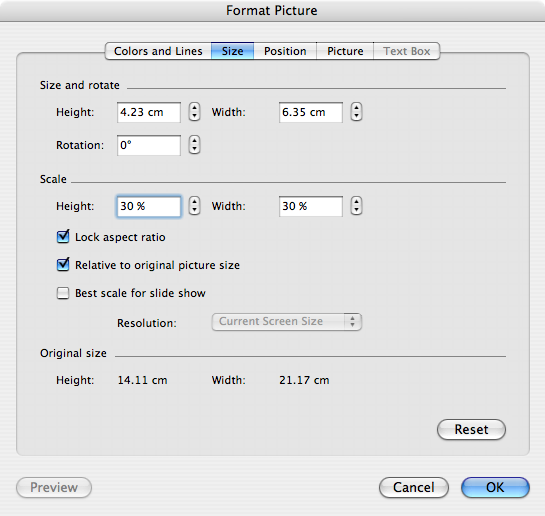
\includegraphics[width=0.6\textwidth,bb=0 0 545 516]{formatpicture.png}
   \caption{\protect\progname{PowerPoint}'s ``Format Picture'' dialogue to set scale and rotation.}
   \label{fig:formatpicture}
\end{figure}

In Figure~\ref{fig:rendering} we have attempted to include Figure~\ref{fig:GMT_example_20} into a \progname{PowerPoint} presentation. First the \PS\ file was converted to PDF (using \GMTprog{ps2raster}), then loaded into \progname{PowerPoint} and the white background color was made transparent using the formatting toolbar (shown on the left side of Figure~\ref{fig:rendering}). Clearly, when we let \progname{PowerPoint} do the rendering, we do not get the best result:
\begin{enumerate}
\item The anti-aliasing causes the tiles that make up the land to stand out. This is because the anti-aliasing algorithm blurs all edges, even when the tiles join seamlessly.
\item The background color was assumed to be white, hence the text is ``smoothed'' using gray shades. Instead, shades of blue which would be appropriate for the background we are using.
\end{enumerate}

On the central column of Figure~\ref{fig:rendering} we have included PNG versions of a portion of the same example. This shows the workings of anti-aliasing and different resolutions. All samples were obtained with \progname{convert}. The one on the top uses all default settings, resulting in an anti-aliased image at 72 dpi resolution (very much like the PDF included directly into \progname{PowerPoint}).

Just switching anti-aliasing off (middle) is clearly not an option either. It is true that we got rid of the gray blurring and the seams between the tiles, but without anti-aliasing the image becomes very blocky. The solution is to render the image at a higher resolution (e.g., 300 dpi) without anti-aliasing and then shrink the image to the appropriate size (bottom of the central column in Figure~\ref{fig:rendering}). The scaling, rotation as well as the selection of the transparent color can be accomplished through the ``Formatting'' tool bar and the ``Format Picture'' dialogue box of \progname{PowerPoint} (Figure~\ref{fig:formatpicture}), which can be found by double clicking the included image (or selecting and right-clicking or control-clicking on a one-button mouse).

\section{Concluding remarks}

These examples do not constitute endorsements of the products mentioned above; they only represent our limited experience with adding \PS\ to various types of documents.  For other solutions and further help, please post messages to
\htmladdnormallink{gmt-help@lists.hawaii.edu}{mailto:gmt-help@lists.hawaii.edu}.
